\newpage
\section{Simulation Analysis}
\label{sec:simulation}
Since this circuit has a sinusoidal voltage source, the voltage and current values of the various components vary in time. Therefore, we must perform a transient analysis to simulate the circuit's total response. We also ran operating point analysis for both $t<0$ and $t=0$ to determine what the initial conditions were and establish the boundary conditions. Finally, we ran a frequency response analysis of the capacitor voltage and node 6 voltage.
\subsection{Operating Point Analysis}
The tables below show the simulated operating point results for both $t<0$ (where we assume no current is flowing through the capacitor) and t=0 where we shut down the voltage source $V_{s}$ and we replace the capacitor with a voltage source $V_{x}$, in order to determine the equivalent resistor seen through the capacitor.
\begin{table}[!htb]
	\begin{minipage}{.5\linewidth}
	\centering
	\begin{tabular}{ll}
	{\bf Name} & {\bf Value [A or V]} \\ \hline
	@gb[i] & -2.29771e-04\\ \hline
@idd[current] & 1.005042e-03\\ \hline
@r1[i] & 2.191669e-04\\ \hline
@r2[i] & 2.297712e-04\\ \hline
@r3[i] & 1.060424e-05\\ \hline
@r4[i] & 1.185502e-03\\ \hline
@r5[i] & 1.234813e-03\\ \hline
@r6[i] & 9.663347e-04\\ \hline
@r7[i] & 9.663347e-04\\ \hline
v(1) & -9.73914e-01\\ \hline
v(3) & 1.063433e+01\\ \hline
v(4) & 6.382611e+00\\ \hline
v(5) & 6.843347e+00\\ \hline
v(6) & 7.067298e+00\\ \hline
v(7) & 1.953900e+00\\ \hline
v(8) & 6.875344e+00\\ \hline
v(9) & 0.000000e+00\\ \hline

	\end{tabular}
	\caption{Operating point analysis for $t<0$. A variable preceded by @ is of type {\em current} other variables are of type {\it voltage} and expressed in Volt.}
	\label{tab:1}
  	\end{minipage}
  	\hfill
	\begin{minipage}{.5\linewidth}
	\centering
  	\begin{tabular}{ll}
   	{\bf Name} & {\bf Value [A or V]} \\ \hline
   	\input{op2_tab}
	\end{tabular}
	\caption{Operating point analysis for $t=0$. A variable preceded by @ is of type {\em current} and expressed in Ampere; other variables are of type {\it voltage} and expressed in Volt.}
	\label{tab:2}
	\end{minipage}
\end{table}

Table ~\ref{tab:1} shows the simulated node voltages and branch currents for $t<0$. Table ~\ref{tab:2} gives us the current flowing through our voltage source, $V_{x}$. With the voltage source value calculated in the previous operating poing simulation, we can now calculate the equivalent resistance, $R_{eq}$, and characteristic time, $\tau$:

\begin{gather*}
  R_{eq} = \frac{V_x}{@V_c[i]} \Leftrightarrow R_{eq} = \frac{8.548722}{2.80822e-03} \Leftrightarrow R_{eq} = 3044.178163 Ohm
\end{gather*}

\begin{gather*}
  \tau = R_{eq} \times C \Leftrightarrow \tau = (3044.178163*C)   s
\end{gather*}

\newpage
\subsection{Natural response}
In this section we simulate the natural response of the circuit in the [0,20] ms time interval using the transient analysis simulation in NGSpice and the computations from the previous section.
\begin{figure}[!h] \centering
\includegraphics[width=0.6\linewidth]{natura.pdf}
\caption{Simulated natural response for $V_{6}$ node voltage.}
\label{fig:natura}
\end{figure}
\newpage
\subsection{Natural and forced response}
We repeat the previous step now with the sinusoidal voltage source $V_{s}(t)$ considering a frequency of 1kHz. Below is the plot for both the stimulus and the response:
\begin{figure}[!h] \centering
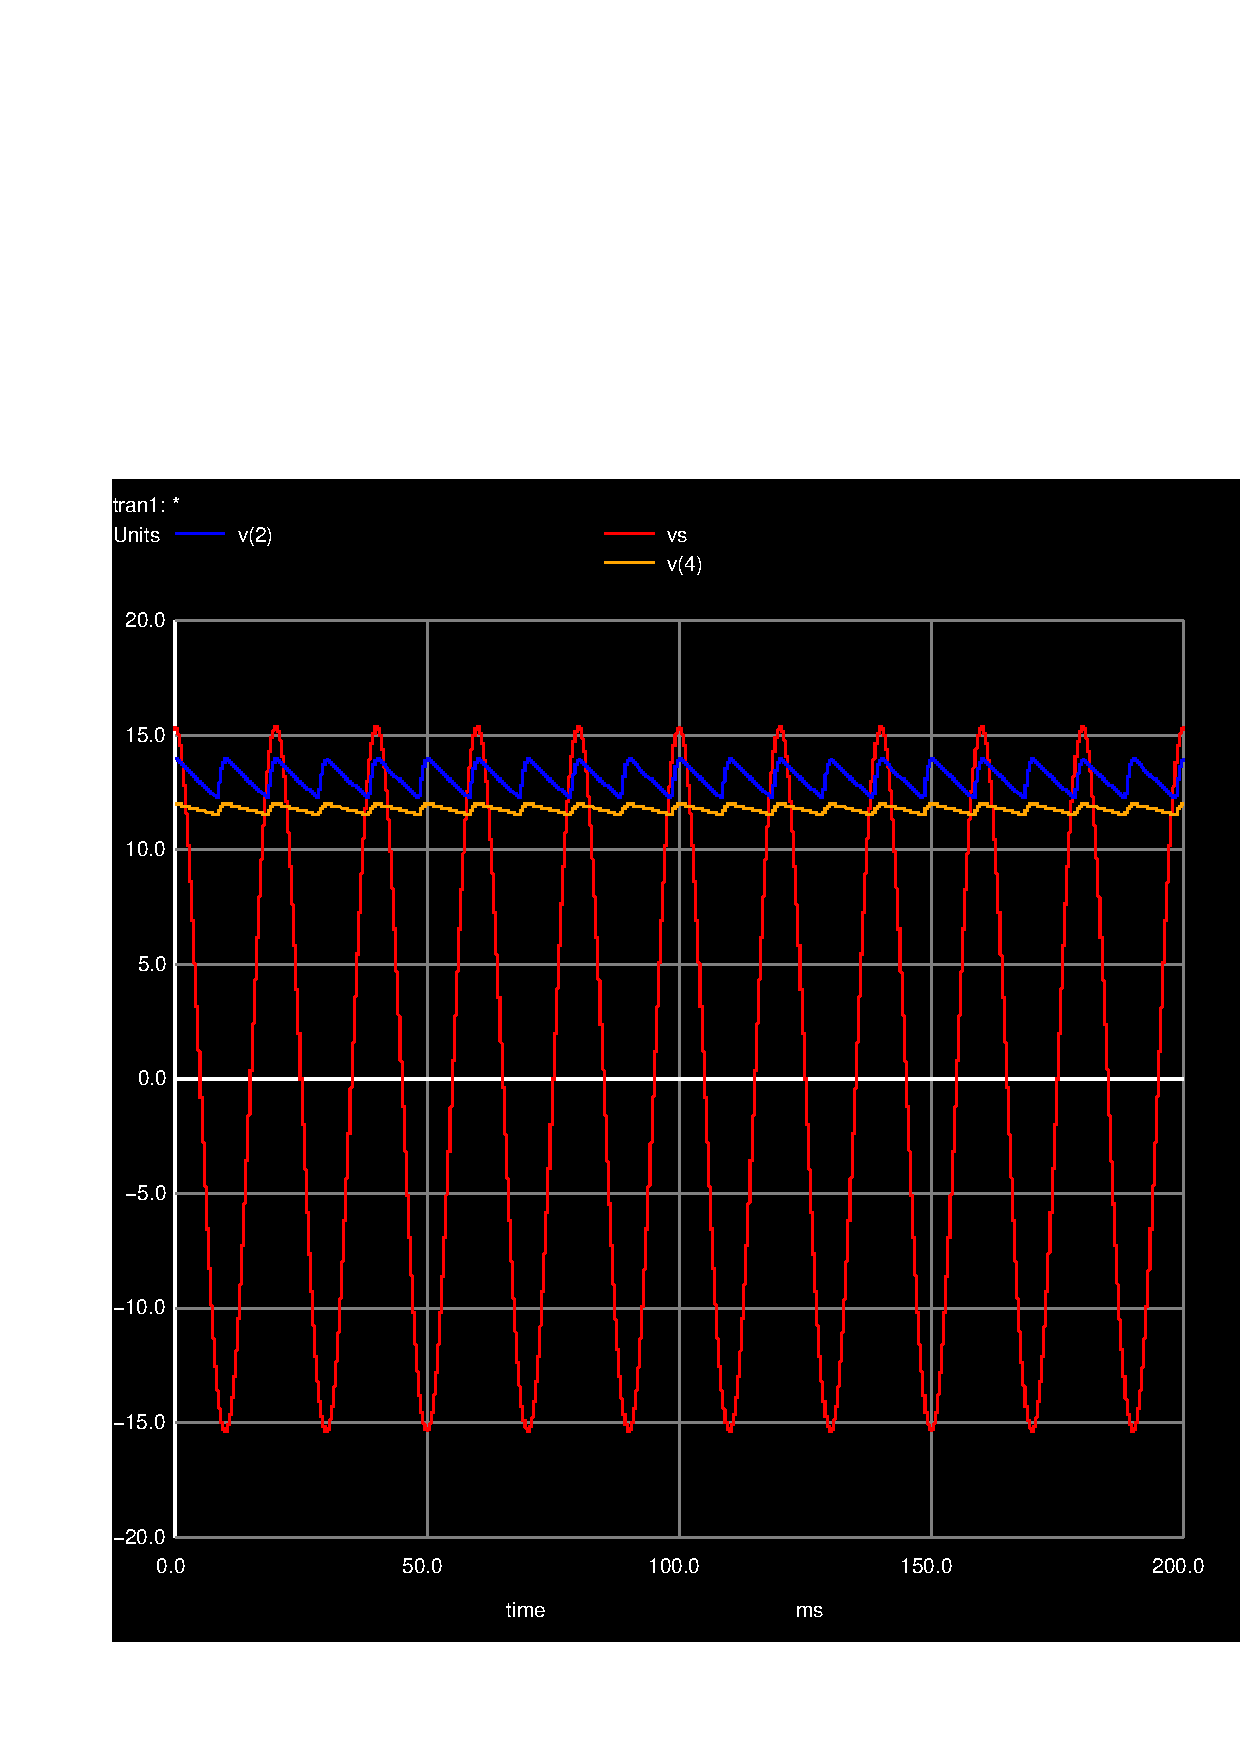
\includegraphics[width=0.6\linewidth]{total.pdf}
\caption{Simulated response for $V_{6}$ node voltage and stimulated voltage $V_{S}$.}
\label{fig:total}
\end{figure}
\newpage
\subsection{Frequency response}
We simulated the frequency response to the voltage source $V_{s}$, both in node 6 and in the capacitor itself, in NGSpice, and we plotted the magnitude, in dB, and phase, in degrees, of the three voltages in relation of course to a variation of frequency. The frequency varies from 0.1 Hz to 1MHz. Analysing figures ~\ref{fig:magnitude} and ~\ref{fig:phase}, they confirm what we foresaw in the theoretical analysis. The various reasons on why certain voltage parameters vary or are equivalent are laid out and explained in the $Frequency$ $Response$ subsection of the theoretical analysis.
\begin{figure}[!h] \centering
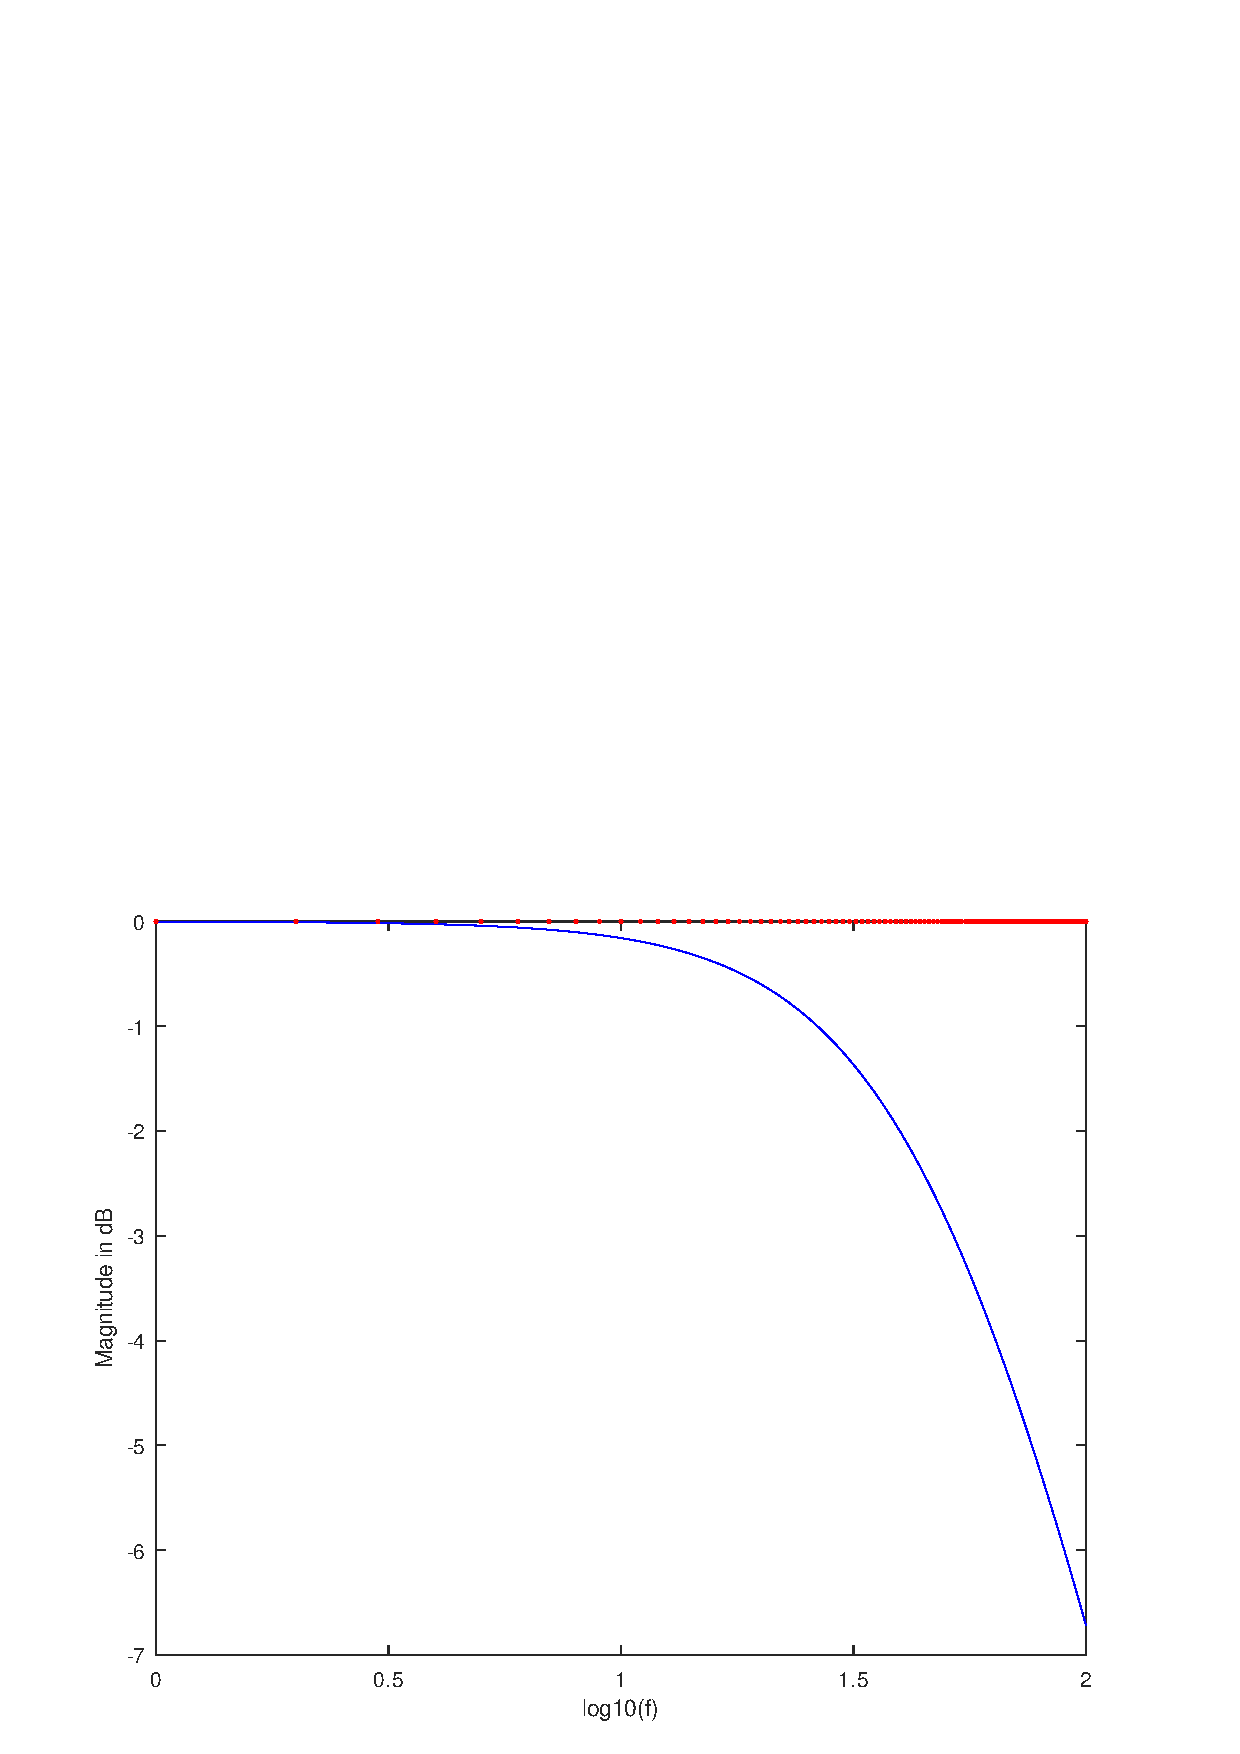
\includegraphics[width=0.6\linewidth]{magnitude.pdf}
\caption{Magnitude of $V_{s}$, $V_{c}$ and $V_{6}$ as a function of frequency}
\label{fig:magnitude}
\end{figure}
\begin{figure}[h] \centering
\includegraphics[width=0.6\linewidth]{phase.pdf}
\caption{Phase of $V_{s}$, $V_{c}$ and $V_{6}$ as a function of frequency}
\label{fig:phase}
\end{figure}
\par
